% !TeX root=../../../main.tex

\chapter{مقدمه}
% دستور زیر باعث عدم‌نمایش شماره صفحه در اولین صفحهٔ این فصل می‌شود.
%\thispagestyle{empty}

\gls{tumor}
از رشد غیر طبیعی سلول با احتمال حمله یا گسترش به سایر قسمت‌های بدن تشکیل می‌شود. \glspl{malignanttumor} معمولاً \gls{cancer} نامیده می‌شوند. سرطان علل مختلفی از جمله تغییرات ژنتیکی، آلودگی محیط زیست یا انتخاب‌های نادرست در سبک زندگی دارد. یک تومور ممکن است از زیرجمعیت‌های سلولی با تغییرات ژنومی‌مشخص تشکیل شده باشد، این پدیده \gls{tumorheterogeneity} نامیده می‌شود. \gls{tumorheterogeneity} احتمالاً برای درمان سرطان و کشف نشانگر زیستی، به ویژه در روش‌های درمانی هدفمند، تأثیراتی خواهد داشت 
\cite{fisher2013cancer}.
درمان‌های فعلی، سرطان را به عنوان یک بیماری همگن درمان می‌کنند
\cite{sun2015intra}.

دارو‌های هدفمند در برابر زیرجمعیت‌های تک یا چند سلولی با \gls{oncogene} جهش‌یافته که آن‌ها را هدف قرار می‌دهند، تولید شده اند، در حالی که آن دسته از زیرجمعیت‌های سلولی که هیچ گونه تاثیری از دارو‌های به واسطه جهش خود، نمی‌گیرند بدون درمان باقی مانده و ممکن است منجر به عود مجدد تومور یا عدم درمان تومور می‌شوند. این زیرجمعیت‌های سلولی بدون درمان ممکن است منجر به پیشرفت تومور پس از درمان دارویی شوند \cite{fisher2013cancer}. به عنوان مثال، رشد مجدد سلول‌های تومورزا در سرطان \gls{colorectalcarcinoma} سرطان پستان و \gls{glioblastomas} پس از تابش یا درمان سیکلوفسفامید مشاهده شده است \cite{sun2015intra}. بنابراین، مطالعه روند رشد تومور و ناهمگنی آن تأثیرات زیادی بر تشخیص و درمان سرطان دارد. 


تومور‌ها می‌توانند خوش‌خیم، بدخیم و دارای رفتاری نامشخص یا ناشناخته باشند \cite{neoplasms}. تومور‌های خوش خیم شامل \glspl{uterinefibroid} و \glspl{melanocyticnevi} است. آن‌ها محدود و \gls{local} هستند و به سرطان تبدیل نمی‌شوند \cite{neoplasia}. \glspl{potentiallymalignanttumor} شامل \gls{carcinomainsitu} هستند. آن‌ها به سایر بافت‌ها حمله نکرده و از بین نمی‌روند اما ممکن است به سرطان تبدیل شوند \cite{canceractivity1}. تومور‌های بدخیم را معمولاً سرطان می‌نامند. آن‌ها به بافت اطراف حمله کرده و از بین می‌روند، ممکن است \gls{metastases} ایجاد کنند و اگر درمان نشوند یا به درمان پاسخ ندهند، کشنده خواهد بود \cite{canceractivity1}. 

\gls{tumorheterogeneity} توضیح می‌دهد که تومور بیش از یک نوع سلول شامل می‌شود. انواع مختلف سلول‌های داخل تومور دارای ویژگی‌های مورفولوژیکی و فیزیولوژیکی متمایزی مانند گیرنده‌های سطح سلول، 
\gls{proliferative}
و 
\gls{angiogenic} هستند. ناهمگنی تومور می‌تواند بین تومور‌ها (ناهمگنی بین توموری) و یا درون تومور‌ها (ناهمگنی درون توموری) رخ دهد. به طور گسترده‌ای پذیرفته شده است که توسعه تومور یک روند تکاملی است \cite{birbrair2014type}، و \gls{spontaneous} معمولاً از یک سلول منشأ می‌گیرند و گروهی از سلول‌ها را تشکیل می‌شوند که در نهایت یک توده را شکل می‌دهند. 

دو مدل برای ناهمگنی تومور وجود دارد (شکل \ref{fig:ch_intr:tumorheterogenety}). یک مدل تشکیل سرطان از طریق سلول‌های بنیادی بوده که قابلیت ارث‌بری ندارند و مدل دیگر تشکیل سرطان از طریق تکامل \gls{clonal} بوده که قابلیت ارثبری دارد. \cite{birbrair2014type}. مفهوم سلول‌های بنیادی سرطانی بیان می‌کند که رشد و پیشرفت بسیاری از تومور‌ها توسط کسری کمی‌از سلول‌ها کنترل می‌شود و اکثر سلول‌های موجود در تومور محصولات تمایز غیر طبیعی سلول‌های بنیادی سرطانی هستند \cite{birbrair2014type}. بنابراین، برای توصیف و از بین بردن سلول‌های بدخیم در تومورها، لازم است که بر بخش کوچکی از سلول‌های تومورزا تمرکز کنیم \cite{handa2011redox}. مفهوم تکامل کلونی بیان می‌کند که تومور از یک سلول طبیعی ژنتیکی بوجود می‌آید که به تعداد زیادی سلول تبدیل می‌شود. در این تکامل، جهش‌های تصادفی به طور مداوم تولید می‌شوند و در نهایت تومور حاصل میلیارد‌ها سلول بدخیم است که حاصل از تجمع تعداد زیادی جهش است\cite{halford2005o6}. تکامل تومور به عنوان توالی پیدرپی گسترش کلونی توصیف می‌شود، که در آن در هر حالت جدید یک رویداد جهش اضافی ایجاد می‌شود \cite{birbrair2014type}. 

\begin{figure}[!ht]
	\centerline{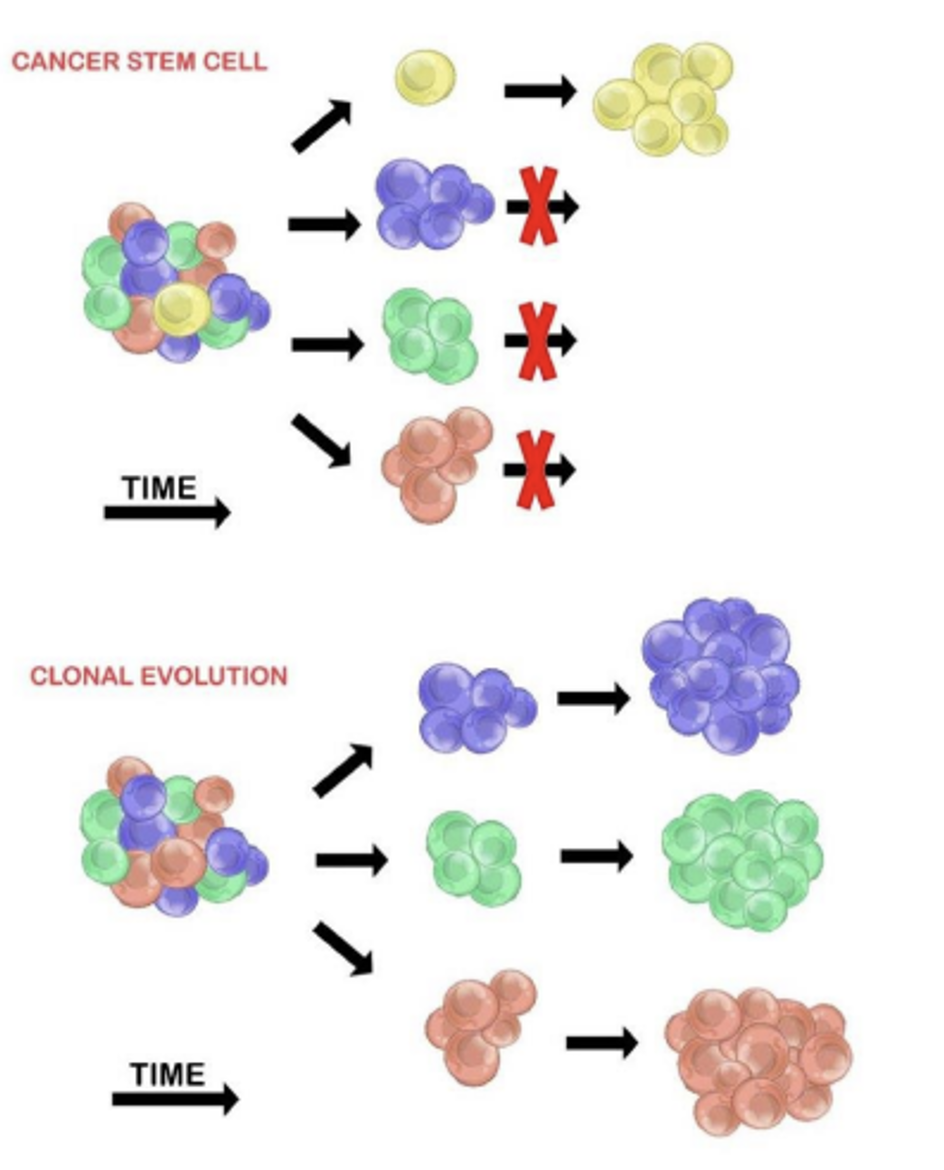
\includegraphics[width=10cm]{chaps/int/tumorheterogenety}}
	\caption{دو مدل برای ناهمگونی تومور}
	\label{fig:ch_intr:tumorheterogenety}
\end{figure}

یکی از توالی‌های پی در پی گسترش کلونی، یک مدل خطی از جانشینی کلونی است، جایی که جهش‌های متوالی پیدرپی باعث ایجاد توالی خطی از مجموعه‌های گسترش کلون می‌شوند و منجر به رشد کلون می‌شوند \cite{birbrair2014type}. مورد دیگر یک مدل چند کلونی از پیشرفت تومور است، که در آن یک سلول منفرد از طریق مکانیزم تقسیم به چندین زیرکلون گسترش می‌یابد \cite{lee2011promoter}. این مدل بیش از مدل خطی با ناهمگنی تومور مرتبط است. جهش‌های اکتسابی منجر به افزایش بی ثباتی ژنومی با هر نسل متوالی می‌شود \cite{cooper1992elements}. 

تومرهای
\gls{heterogenetic}
که متشکل از چندین کلون هستند، می‌توانند حساسیت‌های مختلفی را نسبت به \glspl{cytotoxic} در نشان دهند. علاوه بر این، می‌زان  ناهمگنی تومور می‌تواند خود به عنوان \gls{biomarker} مورد استفاده قرار گیرد زیرا هر چقدر می‌زان ناهمگنی تومور بیشتر باشد، احتمال حضور کلون‌های مقاوم در برابر درمان بیشتر است \cite{truninger2005immunohistochemical}. دلایل حساسیت‌های مختلف می‌تواند تعاملات بین کلون‌ها باشد که ممکن است اثر درمانی را مهار یا تغییر دهد \cite{birbrair2014type}. تومورهایی با ناهمگنی زیاد، با احتمال بیشتری از کلون‌های گوناگون تشکیل شده است که به درمان مقاوم هستند و ممکن است منجر به عدم موفقیت در درمان شوند. روش‌های نوین درمان تومور‌ها با هدف شخصی‌سازی برنامه‌های درمانی از طریق هدف قرار دادن جمعیت‌های سلولی توموری موجود در یک بیمار، توسعه می‌یابند \cite{fedele2014navigating}. ناهمگنی‌های توموری یکی از عوامل اصلی مقاومت در برابر دارو است و بنابراین، یک عامل بالقوه  در شکست درمان محسوب می‌شود. \cite{fedele2014navigating}. تومور‌ها می‌توانند از راه‌های مختلف به طور همزمان به مقاومت دارویی دست یابند، بنابراین هدف قرار دادن فقط یک مکانیسم مقاومت برای غلبه بر نارسایی درمانی، می‌تواند مزیت درمان‌های هدفمند را محدود کند\cite{burrell2014tumour}. بنابراین، ناهمگنی تومور می‌تواند برای درک توسعه تومور، پیچیدگی ایجاد کند و توسعه روش‌های موفقیت آمیز را با چالش روبرو کند \cite{fedele2014navigating}. مطالعه ناهمگنی تومور می‌تواند منجر به پیشرفت و توسعه روش‌های درمانی شخصی سازی شده شوند و درک ما را از روابط عملکردی بین کلون‌ها در طول درمان افزایش دهند\cite{burrell2014tumour}. برای مطالعه ناهمگنی تومور، بسیاری از ابزار‌های محاسباتی موثر برای تجزیه و تحلیل اطلاعات کلونی تومور و تاریخچه تکامل آن تولید شده است. این ابزار‌ها با استفاده از داده‌های تغییرپذیری ژنتیکی، تولید شده توسط فناوری‌های توالی یابی نسبتاً دقیق، قادر هستند تا ترکیب‌های کلونی تومور و رابطه اجداد بین کلون‌ها نتیجه دهند. این اطلاعات برای درک پیشرفت تومور و کمک به پیشرفت‌های درمانی کارآمد مهم است. 


در ادامه مفاهیم حوزه تحقیق مثل مدل‌های ناهمگنی توموری، روش‌های مختلف توالی‌یابی، ‌روش‌های مختلف ساخت درخت فیلوژنی تومور، مباحث مرتبط به یادگیری عمیق و یادگیری تقویتی به اختصار توضیح داده شد. در فصل سوم تحقیق پیشرو، به بررسی الگوریتم‌هایی که با استفاده از داده‌های توالی‌یابی تکسولی، درخت فیلوژنی تومور را استنباط کرده‌اند پرداخته شد. هر یک از این روش‌ها برای ساخت درخت فیلوژنی به همراه دادگان مورد استفاده، مورد ارزیابی قرار گرفت و در انت‌های فصل سوم مقایس‌های بین روش‌های مختلف صورت گرفت. در فصل چهارم روش پیشنهادی استنباط درخت فیلوژنی بر مبنای یادگیری تقویتی و داده‌های توالی‌یابی تکسولی به تفصیل بیان شده و در فصل پایانی نتایج بدست آمده و مقایسه آن با نتایج پیشین، گزارش شده است. در پایان موضوعات پیشنهادی که در کار‌های آتی در راستای ادامه این پژوهش می‌تواند مورد بررسی قرار گیرند، توضیح داده شد. 






